% Created by tikzDevice version 0.10.1 on 2017-06-14 16:11:18
% !TEX encoding = UTF-8 Unicode
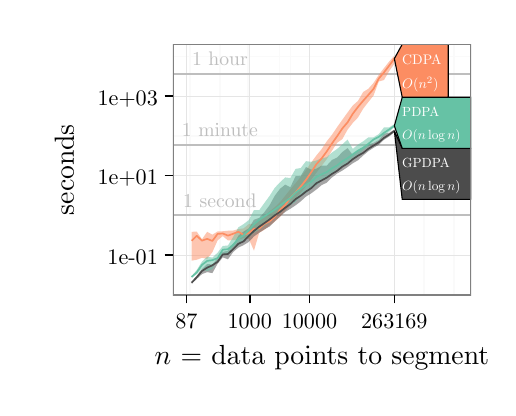
\begin{tikzpicture}[x=1pt,y=1pt]
\definecolor{fillColor}{RGB}{255,255,255}
\path[use as bounding box,fill=fillColor,fill opacity=0.00] (0,0) rectangle (166.22,130.09);
\begin{scope}
\path[clip] (  0.00,  0.00) rectangle (166.22,130.09);
\definecolor{drawColor}{RGB}{255,255,255}
\definecolor{fillColor}{RGB}{255,255,255}

\path[draw=drawColor,line width= 0.6pt,line join=round,line cap=round,fill=fillColor] (  0.00,  0.00) rectangle (166.22,130.09);
\end{scope}
\begin{scope}
\path[clip] ( 52.45, 33.48) rectangle (160.22,124.09);
\definecolor{fillColor}{RGB}{255,255,255}

\path[fill=fillColor] ( 52.45, 33.48) rectangle (160.22,124.09);
\definecolor{drawColor}{gray}{0.98}

\path[draw=drawColor,line width= 0.6pt,line join=round] ( 52.45, 33.60) --
	(160.22, 33.60);

\path[draw=drawColor,line width= 0.6pt,line join=round] ( 52.45, 62.29) --
	(160.22, 62.29);

\path[draw=drawColor,line width= 0.6pt,line join=round] ( 52.45, 90.99) --
	(160.22, 90.99);

\path[draw=drawColor,line width= 0.6pt,line join=round] ( 52.45,119.68) --
	(160.22,119.68);

\path[draw=drawColor,line width= 0.6pt,line join=round] ( 58.65, 33.48) --
	( 58.65,124.09);

\path[draw=drawColor,line width= 0.6pt,line join=round] ( 69.45, 33.48) --
	( 69.45,124.09);

\path[draw=drawColor,line width= 0.6pt,line join=round] ( 91.04, 33.48) --
	( 91.04,124.09);

\path[draw=drawColor,line width= 0.6pt,line join=round] ( 79.59, 33.48) --
	( 79.59,124.09);

\path[draw=drawColor,line width= 0.6pt,line join=round] ( 94.92, 33.48) --
	( 94.92,124.09);

\path[draw=drawColor,line width= 0.6pt,line join=round] (143.30, 33.48) --
	(143.30,124.09);

\path[draw=drawColor,line width= 0.6pt,line join=round] (154.09, 33.48) --
	(154.09,124.09);
\definecolor{drawColor}{gray}{0.90}

\path[draw=drawColor,line width= 0.2pt,line join=round] ( 52.45, 47.94) --
	(160.22, 47.94);

\path[draw=drawColor,line width= 0.2pt,line join=round] ( 52.45, 76.64) --
	(160.22, 76.64);

\path[draw=drawColor,line width= 0.2pt,line join=round] ( 52.45,105.34) --
	(160.22,105.34);

\path[draw=drawColor,line width= 0.2pt,line join=round] ( 80.24, 33.48) --
	( 80.24,124.09);

\path[draw=drawColor,line width= 0.2pt,line join=round] (101.84, 33.48) --
	(101.84,124.09);

\path[draw=drawColor,line width= 0.2pt,line join=round] ( 57.35, 33.48) --
	( 57.35,124.09);

\path[draw=drawColor,line width= 0.2pt,line join=round] (132.50, 33.48) --
	(132.50,124.09);
\definecolor{drawColor}{RGB}{190,190,190}

\path[draw=drawColor,line width= 0.6pt,line join=round] ( 52.45, 62.29) -- (160.22, 62.29);

\path[draw=drawColor,line width= 0.6pt,line join=round] ( 52.45, 87.80) -- (160.22, 87.80);

\path[draw=drawColor,line width= 0.6pt,line join=round] ( 52.45,113.32) -- (160.22,113.32);
\definecolor{fillColor}{RGB}{252,141,98}

\path[fill=fillColor,fill opacity=0.50] ( 59.23, 56.31) --
	( 61.10, 56.41) --
	( 62.98, 53.63) --
	( 64.86, 56.33) --
	( 66.74, 55.29) --
	( 68.62, 56.44) --
	( 70.50, 56.53) --
	( 72.38, 56.71) --
	( 74.26, 56.77) --
	( 76.14, 57.32) --
	( 78.01, 57.55) --
	( 79.89, 59.09) --
	( 81.77, 59.27) --
	( 83.65, 60.25) --
	( 85.53, 61.93) --
	( 87.41, 63.71) --
	( 89.29, 65.22) --
	( 91.17, 67.03) --
	( 93.05, 69.35) --
	( 94.92, 71.70) --
	( 96.80, 73.89) --
	( 98.68, 76.20) --
	(100.56, 78.62) --
	(102.44, 81.34) --
	(104.32, 83.90) --
	(106.20, 86.17) --
	(108.08, 89.06) --
	(109.96, 91.40) --
	(111.83, 94.17) --
	(113.71, 96.82) --
	(115.59, 99.43) --
	(117.47,101.96) --
	(119.35,103.61) --
	(121.23,106.85) --
	(123.11,108.01) --
	(124.99,110.14) --
	(126.87,113.05) --
	(128.74,115.46) --
	(130.62,117.84) --
	(132.50,119.97) --
	(132.50,117.05) --
	(130.62,114.38) --
	(128.74,111.17) --
	(126.87,110.63) --
	(124.99,105.59) --
	(123.11,103.24) --
	(121.23,100.79) --
	(119.35, 97.63) --
	(117.47, 95.66) --
	(115.59, 93.22) --
	(113.71, 89.83) --
	(111.83, 88.50) --
	(109.96, 85.63) --
	(108.08, 82.61) --
	(106.20, 80.12) --
	(104.32, 77.65) --
	(102.44, 75.15) --
	(100.56, 72.82) --
	( 98.68, 70.51) --
	( 96.80, 68.28) --
	( 94.92, 65.92) --
	( 93.05, 63.83) --
	( 91.17, 61.72) --
	( 89.29, 60.00) --
	( 87.41, 58.57) --
	( 85.53, 57.08) --
	( 83.65, 55.93) --
	( 81.77, 49.53) --
	( 79.89, 53.78) --
	( 78.01, 54.02) --
	( 76.14, 53.50) --
	( 74.26, 53.32) --
	( 72.38, 53.21) --
	( 70.50, 54.79) --
	( 68.62, 53.21) --
	( 66.74, 48.97) --
	( 64.86, 46.55) --
	( 62.98, 46.93) --
	( 61.10, 46.23) --
	( 59.23, 45.90) --
	cycle;
\definecolor{fillColor}{RGB}{77,77,77}

\path[fill=fillColor,fill opacity=0.50] ( 59.23, 38.22) --
	( 61.10, 40.44) --
	( 62.98, 42.83) --
	( 64.86, 44.66) --
	( 66.74, 44.55) --
	( 68.62, 46.78) --
	( 70.50, 49.08) --
	( 72.38, 49.48) --
	( 74.26, 51.50) --
	( 76.14, 54.93) --
	( 78.01, 56.41) --
	( 79.89, 57.59) --
	( 81.77, 60.70) --
	( 83.65, 61.34) --
	( 85.53, 63.44) --
	( 87.41, 65.92) --
	( 89.29, 69.35) --
	( 91.17, 71.84) --
	( 93.05, 73.37) --
	( 94.92, 72.43) --
	( 96.80, 76.42) --
	( 98.68, 76.52) --
	(100.56, 79.73) --
	(102.44, 78.79) --
	(104.32, 79.14) --
	(106.20, 80.25) --
	(108.08, 80.26) --
	(109.96, 82.28) --
	(111.83, 83.17) --
	(113.71, 85.16) --
	(115.59, 86.58) --
	(117.47, 84.11) --
	(119.35, 85.53) --
	(121.23, 86.82) --
	(123.11, 87.95) --
	(124.99, 88.45) --
	(126.87, 89.50) --
	(128.74, 91.81) --
	(130.62, 92.09) --
	(132.50, 93.26) --
	(132.50, 92.31) --
	(130.62, 90.78) --
	(128.74, 89.57) --
	(126.87, 87.77) --
	(124.99, 86.69) --
	(123.11, 85.47) --
	(121.23, 83.89) --
	(119.35, 82.17) --
	(117.47, 81.08) --
	(115.59, 79.71) --
	(113.71, 78.46) --
	(111.83, 77.38) --
	(109.96, 75.95) --
	(108.08, 74.09) --
	(106.20, 73.18) --
	(104.32, 71.62) --
	(102.44, 70.21) --
	(100.56, 69.05) --
	( 98.68, 67.34) --
	( 96.80, 65.88) --
	( 94.92, 64.65) --
	( 93.05, 63.48) --
	( 91.17, 61.86) --
	( 89.29, 60.13) --
	( 87.41, 58.25) --
	( 85.53, 57.19) --
	( 83.65, 55.98) --
	( 81.77, 54.64) --
	( 79.89, 52.66) --
	( 78.01, 51.50) --
	( 76.14, 50.63) --
	( 74.26, 49.03) --
	( 72.38, 46.40) --
	( 70.50, 47.08) --
	( 68.62, 44.76) --
	( 66.74, 41.40) --
	( 64.86, 41.75) --
	( 62.98, 41.04) --
	( 61.10, 39.31) --
	( 59.23, 37.60) --
	cycle;
\definecolor{fillColor}{RGB}{102,194,165}

\path[fill=fillColor,fill opacity=0.50] ( 59.23, 40.23) --
	( 61.10, 42.54) --
	( 62.98, 45.54) --
	( 64.86, 47.36) --
	( 66.74, 47.00) --
	( 68.62, 48.76) --
	( 70.50, 51.21) --
	( 72.38, 51.39) --
	( 74.26, 54.47) --
	( 76.14, 57.95) --
	( 78.01, 59.09) --
	( 79.89, 60.55) --
	( 81.77, 64.19) --
	( 83.65, 64.13) --
	( 85.53, 66.73) --
	( 87.41, 69.29) --
	( 89.29, 72.23) --
	( 91.17, 74.19) --
	( 93.05, 75.98) --
	( 94.92, 75.75) --
	( 96.80, 79.06) --
	( 98.68, 79.38) --
	(100.56, 81.85) --
	(102.44, 81.61) --
	(104.32, 82.09) --
	(106.20, 82.89) --
	(108.08, 83.27) --
	(109.96, 84.96) --
	(111.83, 86.27) --
	(113.71, 87.91) --
	(115.59, 89.65) --
	(117.47, 86.27) --
	(119.35, 87.83) --
	(121.23, 89.02) --
	(123.11, 90.45) --
	(124.99, 90.47) --
	(126.87, 91.61) --
	(128.74, 94.03) --
	(130.62, 94.05) --
	(132.50, 95.26) --
	(132.50, 94.21) --
	(130.62, 92.46) --
	(128.74, 91.15) --
	(126.87, 89.18) --
	(124.99, 88.33) --
	(123.11, 87.05) --
	(121.23, 85.70) --
	(119.35, 83.73) --
	(117.47, 82.47) --
	(115.59, 81.40) --
	(113.71, 80.04) --
	(111.83, 79.04) --
	(109.96, 77.51) --
	(108.08, 75.46) --
	(106.20, 74.73) --
	(104.32, 73.12) --
	(102.44, 71.77) --
	(100.56, 70.33) --
	( 98.68, 69.10) --
	( 96.80, 67.11) --
	( 94.92, 65.96) --
	( 93.05, 64.97) --
	( 91.17, 63.04) --
	( 89.29, 61.79) --
	( 87.41, 59.65) --
	( 85.53, 58.43) --
	( 83.65, 57.03) --
	( 81.77, 55.96) --
	( 79.89, 54.27) --
	( 78.01, 53.42) --
	( 76.14, 51.39) --
	( 74.26, 50.63) --
	( 72.38, 48.07) --
	( 70.50, 48.13) --
	( 68.62, 46.40) --
	( 66.74, 42.83) --
	( 64.86, 42.08) --
	( 62.98, 42.83) --
	( 61.10, 41.04) --
	( 59.23, 39.78) --
	cycle;
\definecolor{drawColor}{RGB}{252,141,98}

\path[draw=drawColor,line width= 0.6pt,line join=round] ( 59.23, 53.07) --
	( 61.10, 54.88) --
	( 62.98, 53.13) --
	( 64.86, 53.78) --
	( 66.74, 53.02) --
	( 68.62, 55.57) --
	( 70.50, 55.72) --
	( 72.38, 54.95) --
	( 74.26, 55.62) --
	( 76.14, 56.36) --
	( 78.01, 55.24) --
	( 79.89, 55.87) --
	( 81.77, 57.41) --
	( 83.65, 57.49) --
	( 85.53, 59.16) --
	( 87.41, 60.08) --
	( 89.29, 61.78) --
	( 91.17, 64.16) --
	( 93.05, 66.01) --
	( 94.92, 68.66) --
	( 96.80, 70.54) --
	( 98.68, 72.71) --
	(100.56, 75.08) --
	(102.44, 77.81) --
	(104.32, 80.75) --
	(106.20, 82.83) --
	(108.08, 85.37) --
	(109.96, 88.25) --
	(111.83, 90.88) --
	(113.71, 93.69) --
	(115.59, 95.87) --
	(117.47, 98.97) --
	(119.35,101.44) --
	(121.23,103.68) --
	(123.11,105.79) --
	(124.99,108.00) --
	(126.87,111.70) --
	(128.74,113.91) --
	(130.62,116.37) --
	(132.50,118.90);
\definecolor{drawColor}{gray}{0.30}

\path[draw=drawColor,line width= 0.6pt,line join=round] ( 59.23, 37.91) --
	( 61.10, 39.90) --
	( 62.98, 42.16) --
	( 64.86, 43.37) --
	( 66.74, 44.22) --
	( 68.62, 45.49) --
	( 70.50, 48.16) --
	( 72.38, 48.31) --
	( 74.26, 50.08) --
	( 76.14, 52.01) --
	( 78.01, 52.88) --
	( 79.89, 54.84) --
	( 81.77, 56.64) --
	( 83.65, 58.16) --
	( 85.53, 59.46) --
	( 87.41, 60.80) --
	( 89.29, 62.26) --
	( 91.17, 63.52) --
	( 93.05, 65.03) --
	( 94.92, 66.36) --
	( 96.80, 68.12) --
	( 98.68, 69.37) --
	(100.56, 70.86) --
	(102.44, 72.08) --
	(104.32, 73.87) --
	(106.20, 74.89) --
	(108.08, 75.91) --
	(109.96, 77.25) --
	(111.83, 78.37) --
	(113.71, 79.89) --
	(115.59, 80.98) --
	(117.47, 82.57) --
	(119.35, 83.82) --
	(121.23, 84.85) --
	(123.11, 86.34) --
	(124.99, 87.50) --
	(126.87, 88.67) --
	(128.74, 90.26) --
	(130.62, 91.44) --
	(132.50, 92.78);
\definecolor{drawColor}{RGB}{102,194,165}

\path[draw=drawColor,line width= 0.6pt,line join=round] ( 59.23, 40.01) --
	( 61.10, 41.66) --
	( 62.98, 44.39) --
	( 64.86, 45.81) --
	( 66.74, 46.07) --
	( 68.62, 46.82) --
	( 70.50, 49.86) --
	( 72.38, 50.04) --
	( 74.26, 51.67) --
	( 76.14, 53.83) --
	( 78.01, 55.06) --
	( 79.89, 56.95) --
	( 81.77, 59.02) --
	( 83.65, 60.66) --
	( 85.53, 61.85) --
	( 87.41, 63.17) --
	( 89.29, 64.32) --
	( 91.17, 65.76) --
	( 93.05, 67.22) --
	( 94.92, 68.54) --
	( 96.80, 70.45) --
	( 98.68, 71.88) --
	(100.56, 73.31) --
	(102.44, 74.39) --
	(104.32, 76.12) --
	(106.20, 77.09) --
	(108.08, 77.91) --
	(109.96, 79.28) --
	(111.83, 80.29) --
	(113.71, 81.85) --
	(115.59, 82.92) --
	(117.47, 84.31) --
	(119.35, 85.66) --
	(121.23, 86.72) --
	(123.11, 88.11) --
	(124.99, 89.70) --
	(126.87, 90.62) --
	(128.74, 92.08) --
	(130.62, 93.31) --
	(132.50, 94.60);
\definecolor{drawColor}{RGB}{190,190,190}

\node[text=drawColor,anchor=base,inner sep=0pt, outer sep=0pt, scale=  0.71] at ( 69.45, 65.23) {1 second};

\node[text=drawColor,anchor=base,inner sep=0pt, outer sep=0pt, scale=  0.71] at ( 69.45, 90.74) {1 minute};

\node[text=drawColor,anchor=base,inner sep=0pt, outer sep=0pt, scale=  0.71] at ( 69.45,116.26) {1 hour};
\end{scope}
\begin{scope}
\path[clip] ( 52.45, 33.48) rectangle (160.22,124.09);
\definecolor{drawColor}{RGB}{0,0,0}
\definecolor{fillColor}{gray}{0.30}

\path[draw=drawColor,line width= 0.4pt,line join=round,line cap=round,fill=fillColor] (132.50, 92.78) --
	(135.35, 86.47) --
	(160.22, 86.47) --
	(160.22, 68.02) --
	(135.35, 68.02) --
	cycle;
\definecolor{fillColor}{RGB}{102,194,165}

\path[draw=drawColor,line width= 0.4pt,line join=round,line cap=round,fill=fillColor] (132.50, 94.60) --
	(135.35,104.93) --
	(160.22,104.93) --
	(160.22, 86.47) --
	(135.35, 86.47) --
	cycle;
\definecolor{fillColor}{RGB}{252,141,98}

\path[draw=drawColor,line width= 0.4pt,line join=round,line cap=round,fill=fillColor] (132.50,118.90) --
	(135.35,124.09) --
	(151.98,124.09) --
	(151.98,104.93) --
	(135.35,104.93) --
	cycle;
\definecolor{drawColor}{RGB}{255,255,255}

\node[text=drawColor,anchor=base west,inner sep=0pt, outer sep=0pt, scale=  0.48] at (135.35, 79.42) {GPDPA};

\node[text=drawColor,anchor=base west,inner sep=0pt, outer sep=0pt, scale=  0.48] at (135.35, 71.10) {$O(n \log n)$};

\node[text=drawColor,anchor=base west,inner sep=0pt, outer sep=0pt, scale=  0.48] at (135.35, 97.87) {PDPA};

\node[text=drawColor,anchor=base west,inner sep=0pt, outer sep=0pt, scale=  0.48] at (135.35, 89.55) {$O(n \log n)$};

\node[text=drawColor,anchor=base west,inner sep=0pt, outer sep=0pt, scale=  0.50] at (135.35,116.76) {CDPA};

\node[text=drawColor,anchor=base west,inner sep=0pt, outer sep=0pt, scale=  0.50] at (135.35,108.12) {$O(n^2)$};
\definecolor{drawColor}{gray}{0.50}

\path[draw=drawColor,line width= 0.6pt,line join=round,line cap=round] ( 52.45, 33.48) rectangle (160.22,124.09);
\end{scope}
\begin{scope}
\path[clip] (  0.00,  0.00) rectangle (166.22,130.09);
\definecolor{drawColor}{RGB}{0,0,0}

\node[text=drawColor,anchor=base east,inner sep=0pt, outer sep=0pt, scale=  0.80] at ( 47.05, 44.64) {1e-01};

\node[text=drawColor,anchor=base east,inner sep=0pt, outer sep=0pt, scale=  0.80] at ( 47.05, 73.33) {1e+01};

\node[text=drawColor,anchor=base east,inner sep=0pt, outer sep=0pt, scale=  0.80] at ( 47.05,102.03) {1e+03};
\end{scope}
\begin{scope}
\path[clip] (  0.00,  0.00) rectangle (166.22,130.09);
\definecolor{drawColor}{RGB}{0,0,0}

\path[draw=drawColor,line width= 0.6pt,line join=round] ( 49.45, 47.94) --
	( 52.45, 47.94);

\path[draw=drawColor,line width= 0.6pt,line join=round] ( 49.45, 76.64) --
	( 52.45, 76.64);

\path[draw=drawColor,line width= 0.6pt,line join=round] ( 49.45,105.34) --
	( 52.45,105.34);
\end{scope}
\begin{scope}
\path[clip] (  0.00,  0.00) rectangle (166.22,130.09);
\definecolor{drawColor}{RGB}{0,0,0}

\path[draw=drawColor,line width= 0.6pt,line join=round] ( 80.24, 30.48) --
	( 80.24, 33.48);

\path[draw=drawColor,line width= 0.6pt,line join=round] (101.84, 30.48) --
	(101.84, 33.48);

\path[draw=drawColor,line width= 0.6pt,line join=round] ( 57.35, 30.48) --
	( 57.35, 33.48);

\path[draw=drawColor,line width= 0.6pt,line join=round] (132.50, 30.48) --
	(132.50, 33.48);
\end{scope}
\begin{scope}
\path[clip] (  0.00,  0.00) rectangle (166.22,130.09);
\definecolor{drawColor}{RGB}{0,0,0}

\node[text=drawColor,anchor=base,inner sep=0pt, outer sep=0pt, scale=  0.80] at ( 80.24, 21.46) {1000};

\node[text=drawColor,anchor=base,inner sep=0pt, outer sep=0pt, scale=  0.80] at (101.84, 21.46) {10000};

\node[text=drawColor,anchor=base,inner sep=0pt, outer sep=0pt, scale=  0.80] at ( 57.35, 21.46) {87};

\node[text=drawColor,anchor=base,inner sep=0pt, outer sep=0pt, scale=  0.80] at (132.50, 21.46) {263169};
\end{scope}
\begin{scope}
\path[clip] (  0.00,  0.00) rectangle (166.22,130.09);
\definecolor{drawColor}{RGB}{0,0,0}

\node[text=drawColor,anchor=base,inner sep=0pt, outer sep=0pt, scale=  1.00] at (106.33,  8.40) {$n$ = data points to segment};
\end{scope}
\begin{scope}
\path[clip] (  0.00,  0.00) rectangle (166.22,130.09);
\definecolor{drawColor}{RGB}{0,0,0}

\node[text=drawColor,rotate= 90.00,anchor=base,inner sep=0pt, outer sep=0pt, scale=  1.00] at ( 16.66, 78.78) {seconds};
\end{scope}
\end{tikzpicture}
